%
% binomialverteilung.tex -- Abschnitt über Binomialverteilung im Kapitel 5
%
% (c) 2015 Prof Dr Andreas Mueller, Hochschule Rapperswil
%
\subsection{Binomialverteilung} \label{section-binomialverteilung}
\index{Bernoulli-Experiment}
\begin{table}
\renewcommand{\arraystretch}{1.5}
\begin{center}
\begin{tabular}{|l|l|}
\hline
Name&Binomialverteilung\\
\hline
Wahrscheinlichkeit&
\begin{minipage}{3.7in}
\vskip3pt
$\displaystyle P(k)=\binom{n}{k}p^k(1-p)^{n-k}$
\end{minipage}
\\[10pt]
Verteilungsfunktion&
$\displaystyle F(k)=\sum_{i=0}^k\binom{n}{i}p^i(1-p)^{n-i}$
\\[10pt]
Erwartungswert&$\displaystyle np$\\
Varianz&$\displaystyle np(1-p)$\\
\hline
Anwendungen&\begin{minipage}{3.7in}%
\strut
$\bullet$ Anzahl Eintreten eines Bernoulli-Experimentes
\strut
\end{minipage}\\
\hline
\end{tabular}
\end{center}
\caption{Datenblatt der Binomialverteilung\label{datenblatt:binomialverteilung}}
\end{table}
\begin{figure}
\centering
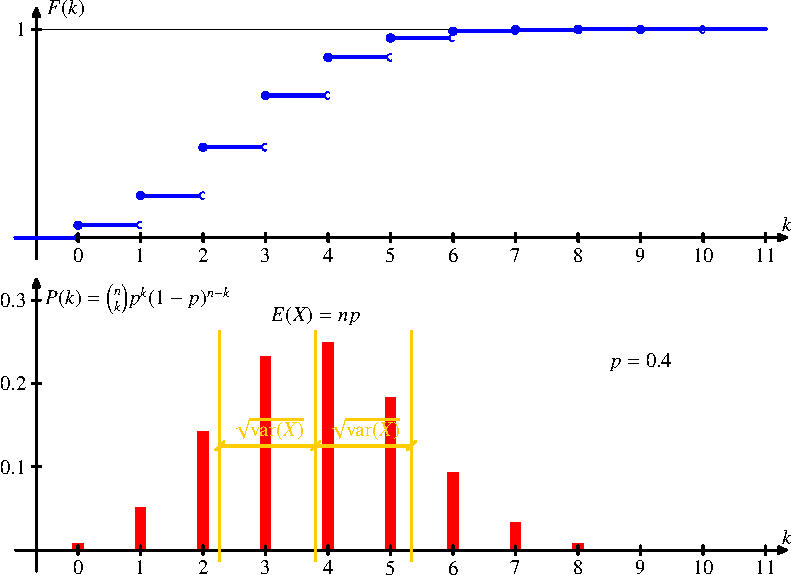
\includegraphics{images/gl-3.pdf}
\caption{Wahrscheinlichkeitsverteilung und Verteilungsfunktion einer
Binomialverteilung mit $p=0.4$ und $n=10$.
\label{binomialgraph}}
\end{figure}

Der Wurf einer M"unze ist der Spezialfall eines Versuches mit
zwei m"oglichen Ausg"angen $\{0,1\}$, bei dem die beiden Ausg"ange als
gleich wahrscheinlich angesehen werden. Es sind durchaus auch
Anwendungsf"alle denkbar, in denen die beiden Ausg"ange unterschiedliche
Wahrscheinlichkeit haben, zum Beispiel $p$ f"ur den Ausgang $1$ und $1-p$
f"ur $0$.
Ein solches Experiment nennt man ein Bernoulliexperiment.

Wir wiederholen jetzt dieses Experiment $n$ mal und betrachten die Ereignisse,
dass in genau $k$ der $n$ F"alle der Ausgang $1$ eingetreten ist,
und $0$ in allen anderen F"allen. Es gibt $\binom{n}{k}$ M"oglichkeiten,
die $k$ $1$-Experimente auszuw"ahlen, und die Kombination, dass genau
dieses Kombination $1$ und $0$ realisiert wird, ist $p^k(1-p)^{n-k}$.
Somit ist die Wahrscheinlichkeit, dass von $n$ Experimenten deren $k$
erfolgreich sind
\[
\binom{n}{k}p^k(1-p)^{n-k}.
\]
Dies ist die Binomialverteilung:
\index{Binomialverteilung}
\begin{definition}
Eine Zufallsvariable mit diskreten Werten $k\in\{0,\dots,n\}$
heisst binomialverteilt zum Parameter $p$, wenn die Wahrscheinlichkeit
des Wertes $k$ 
\[
\binom{n}{k}p^k(1-p)^{n-k}
\]
ist.
\end{definition}

Die Wahrscheinlichkeitsverteilung und die Verteilungsfunktion der
Binomialverteilung ist in Abbildung~\ref{binomialgraph} dargstellt.

\subsubsection{Erwartungswert und Varianz}
\index{Erwartungswert!der Binomialverteilung}
\index{Binomialverteilung!Erwartungswert}
Aus der bekannten Wahrscheinlichkeitsverteilung l"asst sich
Erwartungswert und Varianz berechnen:
\begin{satz}
Eine auf $\{0,\dots,n\}$ zum Parameter $p$ binomialverteilte Zufallsvariable
$X$ hat Erwartungswert
\[
E(X)=pn
\]
und Varianz
\[
\operatorname{var}(X)=np(1-p).
\]
Die maximale Varianz wird erreicht bei $p=\frac12$.
\end{satz}
\index{Varianz!der Binomialverteilung}
\index{Binomialverteilung!Varianz}

\begin{proof}[Beweis] Wir m"ussen die Summen
\begin{eqnarray*}
E(X)&=&\sum_{k=0}^nk\binom{n}{k}p^k(1-p)^{n-k}\\
E(X^2)&=&\sum_{k=0}^nk^2\binom{n}{k}p^k(1-p)^{n-k}
\end{eqnarray*}
berechnen k"onnen. Dazu betrachten wir die Hilfsfunktion
\[
f(x)=(x+y)^n=\sum_{k=0}^n\binom{n}{k}x^ky^{n-k},
\]
offensichtlich erhalten wir die Summe der Wahrscheinlichkeiten aller
binomailverteilten Werte, wenn
wir $x=p$ und $y=(1-p)$ einsetzen.
Die Ableitung nach $x$ gefolgt von Multiplikation mit $x$ liefert
\[
 x\frac{d}{dx}f(x)
=xn(x+y)^{n-1}\\
=\sum_{k=0}\binom{n}{k}kx^ky^{n-k}
\]
Nach Einsetzen von $x=p$ und $y=1-p$ entsteht rechts genau
der gesuchte Erwartungswert, links aber
\[
pn(p+1-p)^{n-1}=pn=\sum_{k=0}^n\binom{n}{k}kp^k(1-p)^{n-k}=E(X).
\]
Erneute Anwendung von $x\frac{d}{dx}$ liefert
\[
xn(x+y)^{n-1}+x^2 n(n-1)x^{n-2}=\sum_{k=0}^n\binom{n}{k}k^2x^ky^{n-k},
\]
und nach Einsetzen der Werte f"ur $x$ und $y$
\[
pn+p^2n(n-1)=\sum_{k=0}^n\binom{n}{k}k^2p^k(1-p)^{n-k}=E(X^2).
\]
Daraus bestimmen wir die Varianz
\[
\operatorname{var}(X)=E(X^2)-E(X)^2=pn+p^2n(n-1)-p^2n^2=p(1-p)n
\]
Die Funktion $p\mapsto np(1-p)$ ist eine quadratische Funktion mit den
Nullstellen $0$ und $1$. Quadratische Funktionen sind symmetrisch um
die Abszisse des Scheitelpunktes, der demzufolge in der Mitte zwischen
den Nullstellen bei $\frac12$ sein muss.
\end{proof}

\subsubsection{Der Grenzwert \texorpdfstring{$n\to\infty$}{n gegen unendlich}}
\index{Binomialverteilung!Normalapproximation}
Was geschieht, wenn die Zahl $n$ der Versuche beliebig vergr"ossert wird?
nat"urlich wird die Zahl der m"oglichen Werte der Zufallsvariable
gr"osser, der Erwartungswert $np$ und die Varianz $np(1-p)$ steigen.
Standardisiert man die Verteilung jedoch, indem man die Zufallsvariable
durch $Y=(X-np)/\sqrt{np(1-p)}$ ersetzt, dann wird die Zufallsvariable $Y$
Erwartungswert $0$ und Varianz $1$ haben. 

Durch die Skalierung r"ucken die m"oglichen Werte von $Y$ n"aher zusammen,
so dass man die Wahrscheinlichkeiten nicht direkt vergleichen kann.
Man kann aber die Verteilungsfunktionen $F_Y$ f"ur verschiedene Werte
von $n$ vergleichen. Aus dem zentralen Grenzwertsatz erh"alt man
jedoch die Aussage, dass die Verteilungsfunktion gegen die
Verteilungsfunktion der Standardnormalverteilung konvergieren wird.
Dieser Spezialfall des zentralen Grenzwertsatzes heisst auch der
Satz von de Moivre und Laplace.

Die Gr"osse $Y=(X-np)/\sqrt{np(1-p)}$ sollte also normalverteilt sein
mit Erwartungswert $0$ und Varianz $1$, aber nat"urlich nur, wenn $p$
tats"achlich die Wahrscheinlichkeit des einen Ausgangs des
Bernoulliexperimentes ist. Daraus l"asst sich jetzt ein Test daf"ur
konstruieren, ob $p$ die Wahrscheinlichkeit des einen Ausgangs eines
Bernoulliexperimentes ist. Ist $p$ n"amlich nicht die richtige
Wahrscheinlichkeit, wird f"ur grosse $Y$ mit grosser Wahrscheinlichkeit
stark von $0$ abweichen, es muss also nur ein Kriterium gefunden werden,
welches angibt, dass die Abweichung zu gross ist, um immer noch daran
zu glauben, dass das $p$ richtig war.

Ein rationales Kriterium l"asst sich mit der $\chi^2$-Verteilung konstruieren.
$Y^2$ ist $\chi^2$-verteilt mit einem Freiheitsgrad.
Die Wahrscheinlichkeit, dass $Y^2$ gr"osser ist als $M$ ist
\[
P(Y^2>M)=\int_M^\infty f_{\frac12,\frac12}(t)\,dt.
\]
Wenn wir also $M$ bestimmen, so dass diese Wahrscheinlichkeit 
zum Beispiel 5\% ist, dann glauben wir nicht mehr, dass $p$ tats"achlich
die Wahrscheinlichkeit des einen Ausgangs ist, sobald $Y^2>M$ wird,
und nur in 5\% aller F"alle werden wir dies zu unrecht tun.
